\chapter{Application development}
Based on the theoretical notions described above, we implement the basics of a facial authentication system that would get real-time feed from the laptop's webcam, detect if there is a face in front of it and upon confirming it is a live one and not a spoof attack, it would search for a face in it's database that is sufficiently similar and assign it's known identity to the face in front of the camera.	


We choose Python as the main code language for multiple reasons ranging from the strong support it has from the opensource community, which puts at our disposal great implementations of the tools we need to create the system we started out with in mind to the well fitting of this language with our pragmatic approach.
\section{Used frameworks}
Having as target the creation of a reliable system, we favor only the most solid frameworks that can be found. This guides us in using Scikit-learn \cite{scikit-learn} in anything related to data analysis as classifiers, metrics or preprocessing methods; this framework being supported, among others, by Google and INRIA(French Institute for Reasearch in Computer Science and Automation). In matters of image processing, from reading an image, getting video feed from webcam to changing the colorspace of an image and applying afine transformations we use OpenCV \cite{opencv_library} as it is designed for computational efficiency with a focus on real-time applications. We also use Scykit-image \cite{scikit-image} for it's implementation of the local binary patterns descriptor. For one of the most important parts of the system, the CNN used for image embedding, we use the OpenFace \cite{amos2016openface} implementation of the FaceNet \cite{SchroffKP15} system.
\section{Application architecture}

\begin{figure}
	\captionsetup{width=15cm,font=small}
	\begin{center}
		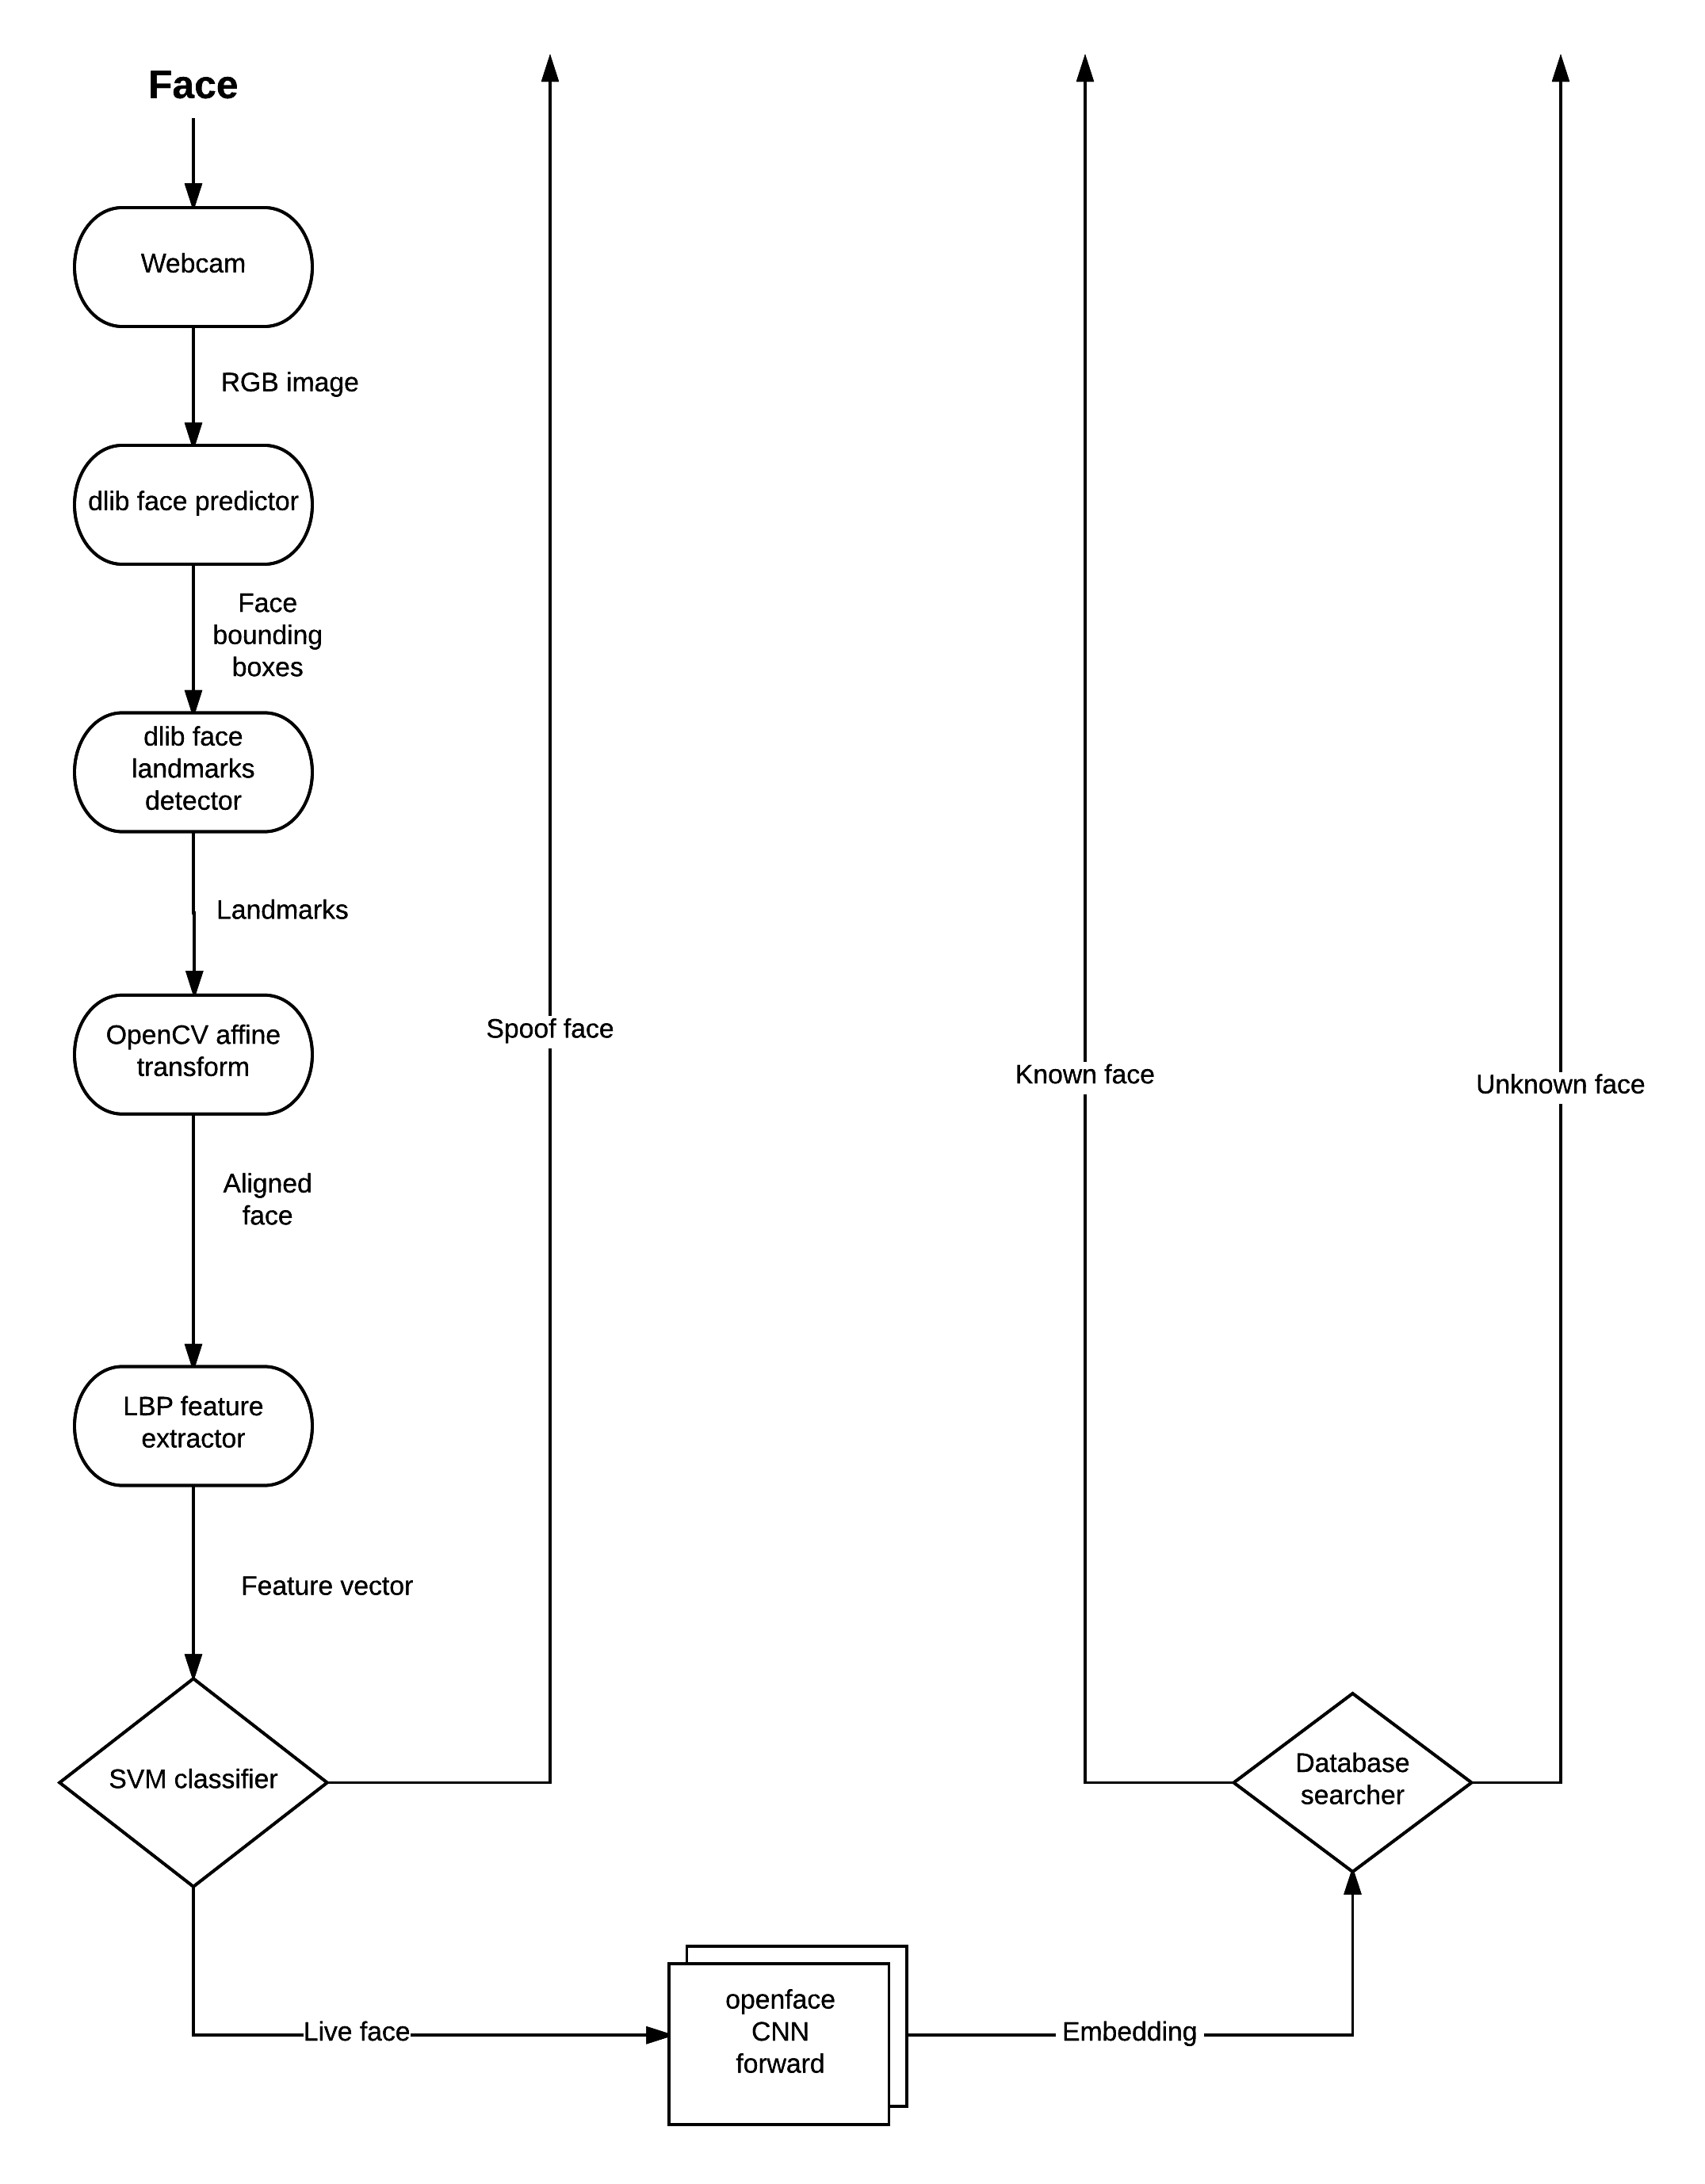
\includegraphics[width=15cm,height=20cm]{application_architecture}
		\caption[Application architecure]{Visual representation of the components of the application}
	\end{center}
	\label{fig:application_architecture}
\end{figure}

The application is designed so that it has a component for each theoretical aspect described above. Therefore, in the application, the stages from reading an image to assigning and identity to a face are as follows: 
\begin{itemize}
	\item we capture a frame using the webcam of the laptop or an external one with the help of opencv framework
	\item we use the dlib \cite{dlib09} face predictor to determine all face bounding boxes in the image
	\item we crop the faces from the full image using each bounding box
	\item we apply the dlib facial landmark detector to the faces obtaining the 68 dimensional array with points corresponding to each landmark
	\item we use the opencv implementation of the affine transformation to align the outer eyes and nose.
	\item on the aligned image of the face, we use our face spoof validator to determine the liveness of it. In order to do so, we implemented the described sliding window method where for each window we employ three LBPs with parameters $(P,R) \in \{(8,1), (8,2), (16,2)\}$. We use the LBP implementation available in the \textit{feature} module of the skimage \cite{scikit-image} framework for which we set the method to "nri\_uniform" representing the non-rotation invariant version of the uniform local binary pattern. A thing to note here is that, even though in the literature the uniform LBP is non-rotation invariant, in the scikit-image \cite{scikit-image} implementation, setting the method to simply uniform results in the computation of a rotation invariant descriptor.
	\begin{figure}[H]
		\captionsetup{width=15cm,font=small}
		\begin{center}
			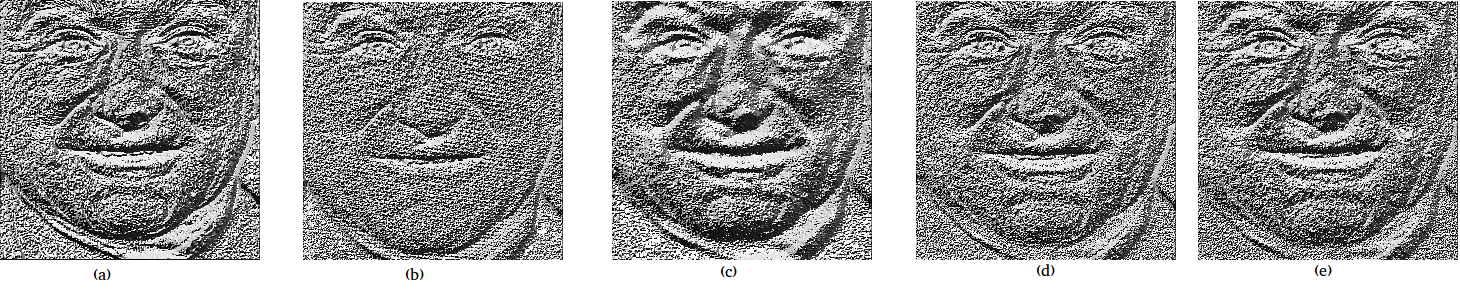
\includegraphics[width=15cm,height=4cm]{visual_results_lbp}
			\caption[LBP feature visualisation on faces]{Here we present the visualisation of the basic LBP with parameters $(P,R) = (8,1)$ for: (a) real image, (b) nexus 5 spoof medium taken with rear camera of a nexus 5, (c) nexus 5 spoof medium taken with front camera of a nexus 5, (d) printed photo spoof medium taken with rear camera of a nexus 5 and (e) printed photo spoof medium taken with front camera of a nexus 5}
		\end{center}
		\label{fig:visual_results_lbp}
	\end{figure}
	\item we use a previously trained SVM with linear kernel to predict the probability of liveness on the computed descriptor. We chose a threshold of $0.6$ to map the probabilities in two classes. If the face is not valid, we make use of the opencv rectangle drawing functionality to put a red bounding box over the spoof face. In the other case, we forward the face through the openface neural network obtaining the 128 dimensional mapping of it.
	\begin{figure}[H]
		\captionsetup{width=15cm,font=small}
		\begin{center}
			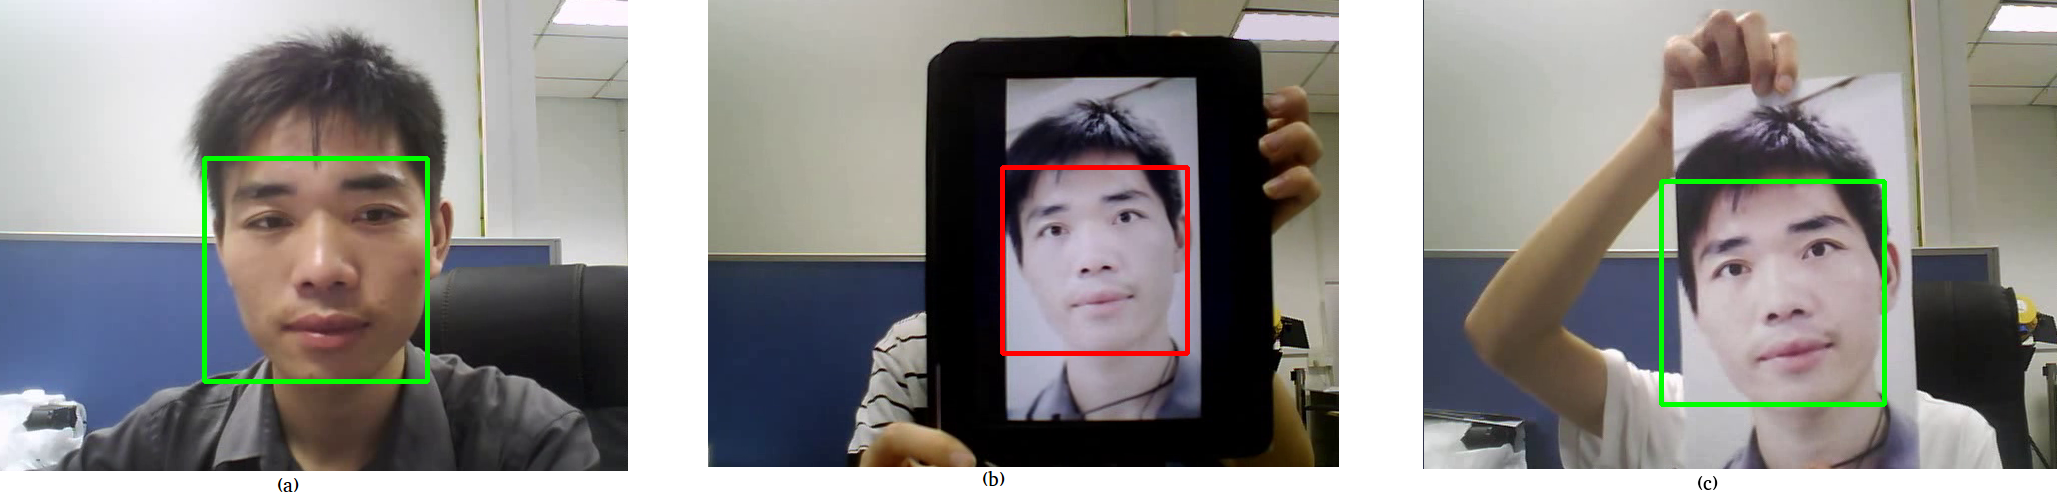
\includegraphics[width=15cm,height=4cm]{spoof_classification_results}
			\caption[Examples on spoof classification]{Here we present the results of the SVM trained on the CASIA database for an example in the test data: (a) is the live face which is correctly classified as being valid, (b) is a spoof face on an IPAD which is correctly classified as being invalid and (c) is a spoof face on a printed paper which is misclassified as being valid}
		\end{center}
		\label{fig:spoof_classification_results}
	\end{figure}
	\item we iterate through the database of known faces and find the face whose representation is closest to the previously computed one. If this minimum distance is smaller than the threshold used for identity matching, we put a green bounding box around the face and append the name corresponding to the matched face. 
\end{itemize} 
\begin{figure}[H]
	\captionsetup{width=15cm,font=small}
	\begin{center}
		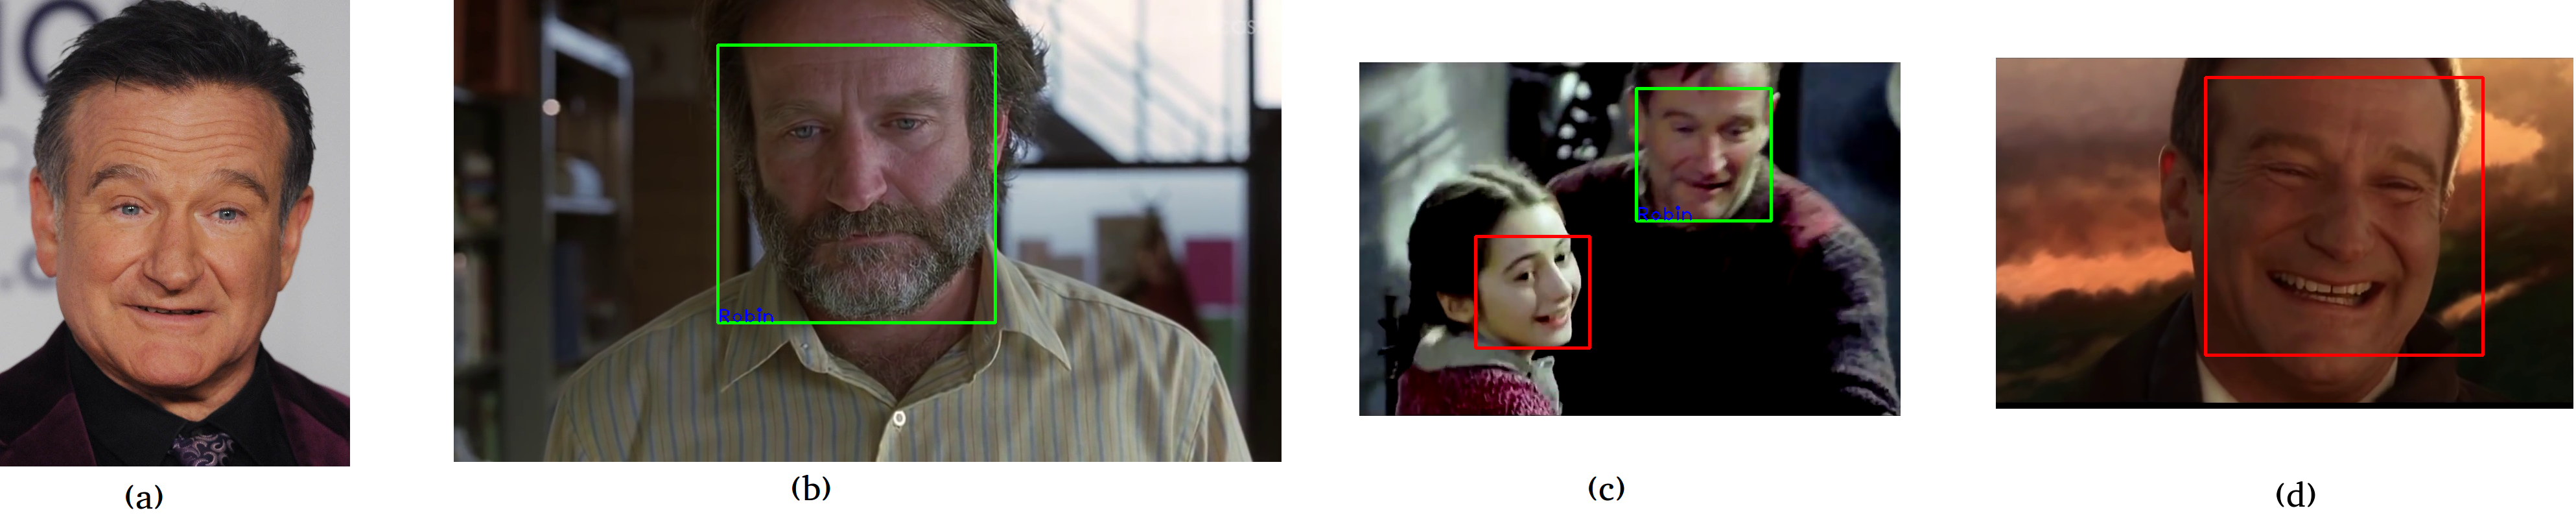
\includegraphics[width=15cm,height=5cm]{face_recognition_results}
		\caption[Examples of face recognition]{We present the results of Openface implementation: (a) is the only picture in the database, (b) is a successfully recognition in adverse conditions (beard), (c) is a successful recognition of Robin Williams while moving and unidentification of the girl, (d) is a fail as the face is not recognized as being Robin Williams given the big smile}
	\end{center}
	\label{fig:face_recognition_examples}
\end{figure}
\section{Running time}
We report the running times of our application on a Lenovo Y50-70 with 8GB of RAM and an Intel CORE i7 4710HQ with a base frequency of 2.50 GHz. The sliding window approach for face detection takes using the dlib python wrapper about 0.25 seconds for an input image of size $480\times640$ that is down-sampled . The face spoof classification takes 0.069 second for a face framed in a bounding box of size $218\times223$, this includes the resizing of the cropped face to a fixed $144\times144$. Face alignment is really fast, taking only 0.003 seconds and passing the aligned face at size $96\times96$ through the network takes only 0.03 seconds. This results in approximately 0.3 seconds for validation, alignment and identification of a face detected in a frame with size $480\times640$.
